\batchmode

 
\documentclass[12pt,oneside]{book}
\RequirePackage{ifthen}


\usepackage[fullpage]{uiucthesis}
\usepackage{graphics}
\usepackage{latexsym}
\usepackage{jeffe}




\usepackage[dvips]{color}


\pagecolor[gray]{.7}

\usepackage[latin1]{inputenc}



\makeatletter
\AtBeginDocument{\makeatletter
\input /home/viblio/quant/web/thesis/thesis-ex.aux
\makeatother
}
\AtBeginDocument{\makeatletter
\input /home/viblio/quant/web/thesis/1-introduction.aux
\makeatother
}
\AtBeginDocument{\makeatletter
\input /home/viblio/quant/web/thesis/2-oracle.aux
\makeatother
}
\AtBeginDocument{\makeatletter
\input /home/viblio/quant/web/thesis/3-graph.aux
\makeatother
}
\AtBeginDocument{\makeatletter
\input /home/viblio/quant/web/thesis/4-general.aux
\makeatother
}
\AtBeginDocument{\makeatletter
\input /home/viblio/quant/web/thesis/5-conclusion.aux
\makeatother
}

\makeatletter
\count@=\the\catcode`\_ \catcode`\_=8 
\newenvironment{tex2html_wrap}{}{}%
\catcode`\<=12\catcode`\_=\count@
\newcommand{\providedcommand}[1]{\expandafter\providecommand\csname #1\endcsname}%
\newcommand{\renewedcommand}[1]{\expandafter\providecommand\csname #1\endcsname{}%
  \expandafter\renewcommand\csname #1\endcsname}%
\newcommand{\newedenvironment}[1]{\newenvironment{#1}{}{}\renewenvironment{#1}}%
\let\newedcommand\renewedcommand
\let\renewedenvironment\newedenvironment
\makeatother
\let\mathon=$
\let\mathoff=$
\ifx\AtBeginDocument\undefined \newcommand{\AtBeginDocument}[1]{}\fi
\newbox\sizebox
\setlength{\hoffset}{0pt}\setlength{\voffset}{0pt}
\addtolength{\textheight}{\footskip}\setlength{\footskip}{0pt}
\addtolength{\textheight}{\topmargin}\setlength{\topmargin}{0pt}
\addtolength{\textheight}{\headheight}\setlength{\headheight}{0pt}
\addtolength{\textheight}{\headsep}\setlength{\headsep}{0pt}
\setlength{\textwidth}{349pt}
\newwrite\lthtmlwrite
\makeatletter
\let\realnormalsize=\normalsize
\global\topskip=2sp
\def\preveqno{}\let\real@float=\@float \let\realend@float=\end@float
\def\@float{\let\@savefreelist\@freelist\real@float}
\def\liih@math{\ifmmode$\else\bad@math\fi}
\def\end@float{\realend@float\global\let\@freelist\@savefreelist}
\let\real@dbflt=\@dbflt \let\end@dblfloat=\end@float
\let\@largefloatcheck=\relax
\let\if@boxedmulticols=\iftrue
\def\@dbflt{\let\@savefreelist\@freelist\real@dbflt}
\def\adjustnormalsize{\def\normalsize{\mathsurround=0pt \realnormalsize
 \parindent=0pt\abovedisplayskip=0pt\belowdisplayskip=0pt}%
 \def\phantompar{\csname par\endcsname}\normalsize}%
\def\lthtmltypeout#1{{\let\protect\string \immediate\write\lthtmlwrite{#1}}}%
\newcommand\lthtmlhboxmathA{\adjustnormalsize\setbox\sizebox=\hbox\bgroup\kern.05em }%
\newcommand\lthtmlhboxmathB{\adjustnormalsize\setbox\sizebox=\hbox to\hsize\bgroup\hfill }%
\newcommand\lthtmlvboxmathA{\adjustnormalsize\setbox\sizebox=\vbox\bgroup %
 \let\ifinner=\iffalse \let\)\liih@math }%
\newcommand\lthtmlboxmathZ{\@next\next\@currlist{}{\def\next{\voidb@x}}%
 \expandafter\box\next\egroup}%
\newcommand\lthtmlmathtype[1]{\gdef\lthtmlmathenv{#1}}%
\newcommand\lthtmllogmath{\dimen0\ht\sizebox \advance\dimen0\dp\sizebox
  \ifdim\dimen0>.95\vsize
   \lthtmltypeout{%
*** image for \lthtmlmathenv\space is too tall at \the\dimen0, reducing to .95 vsize ***}%
   \ht\sizebox.95\vsize \dp\sizebox\z@ \fi
  \lthtmltypeout{l2hSize %
:\lthtmlmathenv:\the\ht\sizebox::\the\dp\sizebox::\the\wd\sizebox.\preveqno}}%
\newcommand\lthtmlfigureA[1]{\let\@savefreelist\@freelist
       \lthtmlmathtype{#1}\lthtmlvboxmathA}%
\newcommand\lthtmlpictureA{\bgroup\catcode`\_=8 \lthtmlpictureB}%
\newcommand\lthtmlpictureB[1]{\lthtmlmathtype{#1}\egroup
       \let\@savefreelist\@freelist \lthtmlhboxmathB}%
\newcommand\lthtmlpictureZ[1]{\hfill\lthtmlfigureZ}%
\newcommand\lthtmlfigureZ{\lthtmlboxmathZ\lthtmllogmath\copy\sizebox
       \global\let\@freelist\@savefreelist}%
\newcommand\lthtmldisplayA{\bgroup\catcode`\_=8 \lthtmldisplayAi}%
\newcommand\lthtmldisplayAi[1]{\lthtmlmathtype{#1}\egroup\lthtmlvboxmathA}%
\newcommand\lthtmldisplayB[1]{\edef\preveqno{(\theequation)}%
  \lthtmldisplayA{#1}\let\@eqnnum\relax}%
\newcommand\lthtmldisplayZ{\lthtmlboxmathZ\lthtmllogmath\lthtmlsetmath}%
\newcommand\lthtmlinlinemathA{\bgroup\catcode`\_=8 \lthtmlinlinemathB}
\newcommand\lthtmlinlinemathB[1]{\lthtmlmathtype{#1}\egroup\lthtmlhboxmathA
  \vrule height1.5ex width0pt }%
\newcommand\lthtmlinlineA{\bgroup\catcode`\_=8 \lthtmlinlineB}%
\newcommand\lthtmlinlineB[1]{\lthtmlmathtype{#1}\egroup\lthtmlhboxmathA}%
\newcommand\lthtmlinlineZ{\egroup\expandafter\ifdim\dp\sizebox>0pt %
  \expandafter\centerinlinemath\fi\lthtmllogmath\lthtmlsetinline}
\newcommand\lthtmlinlinemathZ{\egroup\expandafter\ifdim\dp\sizebox>0pt %
  \expandafter\centerinlinemath\fi\lthtmllogmath\lthtmlsetmath}
\newcommand\lthtmlindisplaymathZ{\egroup %
  \centerinlinemath\lthtmllogmath\lthtmlsetmath}
\def\lthtmlsetinline{\hbox{\vrule width.1em \vtop{\vbox{%
  \kern.1em\copy\sizebox}\ifdim\dp\sizebox>0pt\kern.1em\else\kern.3pt\fi
  \ifdim\hsize>\wd\sizebox \hrule depth1pt\fi}}}
\def\lthtmlsetmath{\hbox{\vrule width.1em\kern-.05em\vtop{\vbox{%
  \kern.1em\kern0.8 pt\hbox{\hglue.17em\copy\sizebox\hglue0.8 pt}}\kern.3pt%
  \ifdim\dp\sizebox>0pt\kern.1em\fi \kern0.8 pt%
  \ifdim\hsize>\wd\sizebox \hrule depth1pt\fi}}}
\def\centerinlinemath{%
  \dimen1=\ifdim\ht\sizebox<\dp\sizebox \dp\sizebox\else\ht\sizebox\fi
  \advance\dimen1by.5pt \vrule width0pt height\dimen1 depth\dimen1 
 \dp\sizebox=\dimen1\ht\sizebox=\dimen1\relax}

\def\lthtmlcheckvsize{\ifdim\ht\sizebox<\vsize 
  \ifdim\wd\sizebox<\hsize\expandafter\hfill\fi \expandafter\vfill
  \else\expandafter\vss\fi}%
\providecommand{\selectlanguage}[1]{}%
\makeatletter \tracingstats = 1 
\providecommand{\Kappa}{\textrm{K}}
\providecommand{\Eta}{\textrm{H}}
\providecommand{\Rho}{\textrm{R}}
\providecommand{\Omicron}{\textrm{O}}
\providecommand{\Iota}{\textrm{J}}
\providecommand{\omicron}{\textrm{o}}
\providecommand{\Mu}{\textrm{M}}
\providecommand{\Tau}{\textrm{T}}
\providecommand{\Epsilon}{\textrm{E}}
\providecommand{\Chi}{\textrm{X}}
\providecommand{\Alpha}{\textrm{A}}
\providecommand{\Beta}{\textrm{B}}
\providecommand{\Zeta}{\textrm{Z}}
\providecommand{\Nu}{\textrm{N}}


\begin{document}
\pagestyle{empty}\thispagestyle{empty}\lthtmltypeout{}%
\lthtmltypeout{latex2htmlLength hsize=\the\hsize}\lthtmltypeout{}%
\lthtmltypeout{latex2htmlLength vsize=\the\vsize}\lthtmltypeout{}%
\lthtmltypeout{latex2htmlLength hoffset=\the\hoffset}\lthtmltypeout{}%
\lthtmltypeout{latex2htmlLength voffset=\the\voffset}\lthtmltypeout{}%
\lthtmltypeout{latex2htmlLength topmargin=\the\topmargin}\lthtmltypeout{}%
\lthtmltypeout{latex2htmlLength topskip=\the\topskip}\lthtmltypeout{}%
\lthtmltypeout{latex2htmlLength headheight=\the\headheight}\lthtmltypeout{}%
\lthtmltypeout{latex2htmlLength headsep=\the\headsep}\lthtmltypeout{}%
\lthtmltypeout{latex2htmlLength parskip=\the\parskip}\lthtmltypeout{}%
\lthtmltypeout{latex2htmlLength oddsidemargin=\the\oddsidemargin}\lthtmltypeout{}%
\makeatletter
\if@twoside\lthtmltypeout{latex2htmlLength evensidemargin=\the\evensidemargin}%
\else\lthtmltypeout{latex2htmlLength evensidemargin=\the\oddsidemargin}\fi%
\lthtmltypeout{}%
\makeatother
\setcounter{page}{1}
\onecolumn

% !!! IMAGES START HERE !!!

\stepcounter{chapter}
\stepcounter{section}
\stepcounter{subsubsection}
\stepcounter{subsubsection}
\stepcounter{section}
\stepcounter{paragraph}
\stepcounter{subsubsection}
\stepcounter{paragraph}
\stepcounter{paragraph}
{\newpage\clearpage
\lthtmlinlinemathA{tex2html_wrap_inline3776}%
$ \sqrt{{N}}$%
\lthtmlinlinemathZ
\lthtmlcheckvsize\clearpage}

{\newpage\clearpage
\lthtmlinlinemathA{tex2html_wrap_inline3779}%
$ \Omega$%
\lthtmlinlinemathZ
\lthtmlcheckvsize\clearpage}

\stepcounter{section}
\stepcounter{subsubsection}
\stepcounter{subsubsection}
\stepcounter{paragraph}
{\newpage\clearpage
\lthtmlinlinemathA{tex2html_wrap_inline3789}%
$ \Complex^{{N}}_{}$%
\lthtmlinlinemathZ
\lthtmlcheckvsize\clearpage}

\stepcounter{paragraph}
{\newpage\clearpage
\lthtmlinlinemathA{tex2html_wrap_inline3794}%
$ \Psi$%
\lthtmlinlinemathZ
\lthtmlcheckvsize\clearpage}

{\newpage\clearpage
\lthtmlinlinemathA{tex2html_wrap_inline3795}%
$ \rangle$%
\lthtmlinlinemathZ
\lthtmlcheckvsize\clearpage}

{\newpage\clearpage
\lthtmlinlinemathA{tex2html_wrap_inline3797}%
$ \Real^{{3}}_{}$%
\lthtmlinlinemathZ
\lthtmlcheckvsize\clearpage}

{\newpage\clearpage
\lthtmlinlinemathA{tex2html_wrap_inline3799}%
$ \hat{{i}}$%
\lthtmlinlinemathZ
\lthtmlcheckvsize\clearpage}

{\newpage\clearpage
\lthtmlinlinemathA{tex2html_wrap_inline3800}%
$ \hat{{j}}$%
\lthtmlinlinemathZ
\lthtmlcheckvsize\clearpage}

{\newpage\clearpage
\lthtmlinlinemathA{tex2html_wrap_inline3801}%
$ \hat{{k}}$%
\lthtmlinlinemathZ
\lthtmlcheckvsize\clearpage}

{\newpage\clearpage
\lthtmlinlinemathA{tex2html_wrap_indisplay3803}%
$\displaystyle \vec{{v}}\,$%
\lthtmlindisplaymathZ
\lthtmlcheckvsize\clearpage}

{\newpage\clearpage
\lthtmlinlinemathA{tex2html_wrap_indisplay3804}%
$\displaystyle \hat{{i}}$%
\lthtmlindisplaymathZ
\lthtmlcheckvsize\clearpage}

{\newpage\clearpage
\lthtmlinlinemathA{tex2html_wrap_indisplay3805}%
$\displaystyle \hat{{j}}$%
\lthtmlindisplaymathZ
\lthtmlcheckvsize\clearpage}

{\newpage\clearpage
\lthtmlinlinemathA{tex2html_wrap_indisplay3806}%
$\displaystyle \hat{{k}}$%
\lthtmlindisplaymathZ
\lthtmlcheckvsize\clearpage}

{\newpage\clearpage
\lthtmlinlinemathA{tex2html_wrap_indisplay3808}%
$\displaystyle \rangle$%
\lthtmlindisplaymathZ
\lthtmlcheckvsize\clearpage}

{\newpage\clearpage
\lthtmlinlinemathA{tex2html_wrap_inline3813}%
$ \langle$%
\lthtmlinlinemathZ
\lthtmlcheckvsize\clearpage}

\stepcounter{subsubsection}
{\newpage\clearpage
\lthtmlinlinemathA{tex2html_wrap_inline3828}%
$ \left\langle\vphantom{ X|Y}\right.$%
\lthtmlinlinemathZ
\lthtmlcheckvsize\clearpage}

{\newpage\clearpage
\lthtmlinlinemathA{tex2html_wrap_inline3829}%
$ \left.\vphantom{ X|Y}\right\rangle$%
\lthtmlinlinemathZ
\lthtmlcheckvsize\clearpage}

{\newpage\clearpage
\lthtmlinlinemathA{tex2html_wrap_inline3830}%
$ \sum_{{i =
0}}^{{N-1}}$%
\lthtmlinlinemathZ
\lthtmlcheckvsize\clearpage}

{\newpage\clearpage
\lthtmlinlinemathA{tex2html_wrap_indisplay3862}%
$\displaystyle \sum_{{k = 0}}^{{N-1}}$%
\lthtmlindisplaymathZ
\lthtmlcheckvsize\clearpage}

\stepcounter{subsubsection}
{\newpage\clearpage
\lthtmlinlinemathA{tex2html_wrap_inline3878}%
$ \Complex^{{2^{N}}}_{}$%
\lthtmlinlinemathZ
\lthtmlcheckvsize\clearpage}

{\newpage\clearpage
\lthtmlinlinemathA{tex2html_wrap_indisplay3880}%
$\displaystyle \left(\vphantom{ \begin{array}{cccc}
	T_{00} & T_{01} & \ldots & T_{0(2^{N}-1)} \\  T_{10} & T_{11} &
	\ldots & T_{2(2^{N}-1)} \\  \vdots & \vdots & & \vdots \\ 
	T_{(2^{N}-1)0} & T_{(2^{N}-1)1} & \ldots &
	T_{(2^{N}-1)(2^{N}-1)}
\end{array}}\right.$%
\lthtmlindisplaymathZ
\lthtmlcheckvsize\clearpage}

{\newpage\clearpage
\lthtmlinlinemathA{tex2html_wrap_indisplay3881}%
$\displaystyle \begin{array}{cccc}
	T_{00} & T_{01} & \ldots & T_{0(2^{N}-1)} \\  T_{10} & T_{11} &
	\ldots & T_{2(2^{N}-1)} \\  \vdots & \vdots & & \vdots \\ 
	T_{(2^{N}-1)0} & T_{(2^{N}-1)1} & \ldots &
	T_{(2^{N}-1)(2^{N}-1)}
\end{array}$%
\lthtmlindisplaymathZ
\lthtmlcheckvsize\clearpage}

{\newpage\clearpage
\lthtmlinlinemathA{tex2html_wrap_indisplay3882}%
$\displaystyle \left.\vphantom{ \begin{array}{cccc}
	T_{00} & T_{01} & \ldots & T_{0(2^{N}-1)} \\  T_{10} & T_{11} &
	\ldots & T_{2(2^{N}-1)} \\  \vdots & \vdots & & \vdots \\ 
	T_{(2^{N}-1)0} & T_{(2^{N}-1)1} & \ldots &
	T_{(2^{N}-1)(2^{N}-1)}
\end{array}}\right)$%
\lthtmlindisplaymathZ
\lthtmlcheckvsize\clearpage}

\stepcounter{subsubsection}
{\newpage\clearpage
\lthtmlinlinemathA{tex2html_wrap_inline3893}%
$ \Real^{{2^{N}}}_{}$%
\lthtmlinlinemathZ
\lthtmlcheckvsize\clearpage}

\stepcounter{subsection}
{\newpage\clearpage
\lthtmlinlinemathA{tex2html_wrap_inline3897}%
$ \in$%
\lthtmlinlinemathZ
\lthtmlcheckvsize\clearpage}

\stepcounter{section}
\stepcounter{section}
{\newpage\clearpage
\lthtmlinlinemathA{tex2html_wrap_inline3907}%
$ \left(\vphantom{\sqrt{N}}\right.$%
\lthtmlinlinemathZ
\lthtmlcheckvsize\clearpage}

{\newpage\clearpage
\lthtmlinlinemathA{tex2html_wrap_inline3909}%
$ \left.\vphantom{\sqrt{N}}\right)$%
\lthtmlinlinemathZ
\lthtmlcheckvsize\clearpage}

{\newpage\clearpage
\lthtmlinlinemathA{tex2html_wrap_inline3918}%
$ \left(\vphantom{\sqrt{\frac{(N-a)b}{(b-a)^{2}}}}\right.$%
\lthtmlinlinemathZ
\lthtmlcheckvsize\clearpage}

{\newpage\clearpage
\lthtmlinlinemathA{tex2html_wrap_inline3919}%
$ \sqrt{{\frac{(N-a)b}{(b-a)^{2}}}}$%
\lthtmlinlinemathZ
\lthtmlcheckvsize\clearpage}

{\newpage\clearpage
\lthtmlinlinemathA{tex2html_wrap_inline3920}%
$ \left.\vphantom{\sqrt{\frac{(N-a)b}{(b-a)^{2}}}}\right)$%
\lthtmlinlinemathZ
\lthtmlcheckvsize\clearpage}

{\newpage\clearpage
\lthtmlinlinemathA{tex2html_wrap_inline3933}%
$ \left(\vphantom{N}\right.$%
\lthtmlinlinemathZ
\lthtmlcheckvsize\clearpage}

{\newpage\clearpage
\lthtmlinlinemathA{tex2html_wrap_inline3934}%
$ \left.\vphantom{N}\right)$%
\lthtmlinlinemathZ
\lthtmlcheckvsize\clearpage}

{\newpage\clearpage
\lthtmlinlinemathA{tex2html_wrap_inline3946}%
$ \left(\vphantom{V}\right.$%
\lthtmlinlinemathZ
\lthtmlcheckvsize\clearpage}

{\newpage\clearpage
\lthtmlinlinemathA{tex2html_wrap_inline3947}%
$ \left.\vphantom{V}\right)$%
\lthtmlinlinemathZ
\lthtmlcheckvsize\clearpage}

{\newpage\clearpage
\lthtmlinlinemathA{tex2html_wrap_inline3954}%
$ \left(\vphantom{\sqrt[4]{N}}\right.$%
\lthtmlinlinemathZ
\lthtmlcheckvsize\clearpage}

{\newpage\clearpage
\lthtmlinlinemathA{tex2html_wrap_inline3955}%
$ \sqrt[4]{{N}}$%
\lthtmlinlinemathZ
\lthtmlcheckvsize\clearpage}

{\newpage\clearpage
\lthtmlinlinemathA{tex2html_wrap_inline3956}%
$ \left.\vphantom{\sqrt[4]{N}}\right)$%
\lthtmlinlinemathZ
\lthtmlcheckvsize\clearpage}

{\newpage\clearpage
\lthtmlinlinemathA{tex2html_wrap_inline3964}%
$ \left(\vphantom{\sqrt[4]{D(f)}}\right.$%
\lthtmlinlinemathZ
\lthtmlcheckvsize\clearpage}

{\newpage\clearpage
\lthtmlinlinemathA{tex2html_wrap_inline3965}%
$ \sqrt[4]{{D(f)}}$%
\lthtmlinlinemathZ
\lthtmlcheckvsize\clearpage}

{\newpage\clearpage
\lthtmlinlinemathA{tex2html_wrap_inline3966}%
$ \left.\vphantom{\sqrt[4]{D(f)}}\right)$%
\lthtmlinlinemathZ
\lthtmlcheckvsize\clearpage}



\newtheorem{theorem}{Theorem}[section]%



\newtheorem{lemma}{Lemma}[section]%



\newtheorem{defi}{Definition}[section]%



\newtheorem{corollary}{Corollary}[section]%

\stepcounter{chapter}
\stepcounter{section}
\stepcounter{subsubsection}
\stepcounter{subsubsection}
{\newpage\clearpage
\lthtmlinlinemathA{tex2html_wrap_inline4058}%
$ \otimes$%
\lthtmlinlinemathZ
\lthtmlcheckvsize\clearpage}

{\newpage\clearpage
\lthtmlinlinemathA{tex2html_wrap_inline4060}%
$ \Complex^{{2^{m}}}_{}$%
\lthtmlinlinemathZ
\lthtmlcheckvsize\clearpage}

{\newpage\clearpage
\lthtmlinlinemathA{tex2html_wrap_inline4063}%
$ \Complex^{{|S|}}_{}$%
\lthtmlinlinemathZ
\lthtmlcheckvsize\clearpage}

{\newpage\clearpage
\lthtmlinlinemathA{tex2html_wrap_inline4077}%
$ \Complex^{{|S|2^{m}}}_{}$%
\lthtmlinlinemathZ
\lthtmlcheckvsize\clearpage}

{\newpage\clearpage
\lthtmlinlinemathA{tex2html_wrap_inline4082}%
$ \lceil$%
\lthtmlinlinemathZ
\lthtmlcheckvsize\clearpage}

{\newpage\clearpage
\lthtmlinlinemathA{tex2html_wrap_inline4083}%
$ \rceil$%
\lthtmlinlinemathZ
\lthtmlcheckvsize\clearpage}

{\newpage\clearpage
\lthtmlinlinemathA{tex2html_wrap_inline4092}%
$ \oplus$%
\lthtmlinlinemathZ
\lthtmlcheckvsize\clearpage}

{\newpage\clearpage
\lthtmlinlinemathA{tex2html_wrap_indisplay4106}%
$\displaystyle \rightarrow$%
\lthtmlindisplaymathZ
\lthtmlcheckvsize\clearpage}

{\newpage\clearpage
\lthtmlinlinemathA{tex2html_wrap_inline4129}%
$\scriptscriptstyle \Omega$%
\lthtmlinlinemathZ
\lthtmlcheckvsize\clearpage}

\stepcounter{subsubsection}
{\newpage\clearpage
\lthtmlinlinemathA{tex2html_wrap_inline4142}%
$ \neq$%
\lthtmlinlinemathZ
\lthtmlcheckvsize\clearpage}

{\newpage\clearpage
\lthtmlinlinemathA{tex2html_wrap_inline4148}%
$ \subseteq$%
\lthtmlinlinemathZ
\lthtmlcheckvsize\clearpage}

{\newpage\clearpage
\lthtmlinlinemathA{tex2html_wrap_indisplay4176}%
$\displaystyle \Omega$%
\lthtmlindisplaymathZ
\lthtmlcheckvsize\clearpage}

{\newpage\clearpage
\lthtmlinlinemathA{tex2html_wrap_indisplay4177}%
$\displaystyle \left(\vphantom{\sqrt{\frac{mm^{\prime}}{ll^{\prime}}}}\right.$%
\lthtmlindisplaymathZ
\lthtmlcheckvsize\clearpage}

{\newpage\clearpage
\lthtmlinlinemathA{tex2html_wrap_indisplay4178}%
$\displaystyle \sqrt{{\frac{mm^{\prime}}{ll^{\prime}}}}$%
\lthtmlindisplaymathZ
\lthtmlcheckvsize\clearpage}

{\newpage\clearpage
\lthtmlinlinemathA{tex2html_wrap_indisplay4179}%
$\displaystyle \left.\vphantom{\sqrt{\frac{mm^{\prime}}{ll^{\prime}}}}\right)$%
\lthtmlindisplaymathZ
\lthtmlcheckvsize\clearpage}

\stepcounter{paragraph}
{\newpage\clearpage
\lthtmlinlinemathA{tex2html_wrap_inline4187}%
$ \left|\vphantom{ 0 }\right.$%
\lthtmlinlinemathZ
\lthtmlcheckvsize\clearpage}

{\newpage\clearpage
\lthtmlinlinemathA{tex2html_wrap_inline4188}%
$ \left.\vphantom{ 0 }\right\rangle$%
\lthtmlinlinemathZ
\lthtmlcheckvsize\clearpage}

{\newpage\clearpage
\lthtmlinlinemathA{tex2html_wrap_inline4195}%
$ \left|\vphantom{ x }\right.$%
\lthtmlinlinemathZ
\lthtmlcheckvsize\clearpage}

{\newpage\clearpage
\lthtmlinlinemathA{tex2html_wrap_inline4196}%
$ \left.\vphantom{ x }\right\rangle$%
\lthtmlinlinemathZ
\lthtmlcheckvsize\clearpage}

{\newpage\clearpage
\lthtmlinlinemathA{tex2html_wrap_indisplay4198}%
$\displaystyle \left(\vphantom{
  \alpha_{x}\left|f(x)\right\rangle
  +
  \beta_{x}|\overline{f(x)}\rangle
}\right.$%
\lthtmlindisplaymathZ
\lthtmlcheckvsize\clearpage}

{\newpage\clearpage
\lthtmlinlinemathA{tex2html_wrap_indisplay4199}%
$\displaystyle \alpha_{{x}}^{}$%
\lthtmlindisplaymathZ
\lthtmlcheckvsize\clearpage}

{\newpage\clearpage
\lthtmlinlinemathA{tex2html_wrap_indisplay4200}%
$\displaystyle \left|\vphantom{f(x)}\right.$%
\lthtmlindisplaymathZ
\lthtmlcheckvsize\clearpage}

{\newpage\clearpage
\lthtmlinlinemathA{tex2html_wrap_indisplay4201}%
$\displaystyle \left.\vphantom{f(x)}\right\rangle$%
\lthtmlindisplaymathZ
\lthtmlcheckvsize\clearpage}

{\newpage\clearpage
\lthtmlinlinemathA{tex2html_wrap_indisplay4202}%
$\displaystyle \beta_{{x}}^{}$%
\lthtmlindisplaymathZ
\lthtmlcheckvsize\clearpage}

{\newpage\clearpage
\lthtmlinlinemathA{tex2html_wrap_indisplay4203}%
$\displaystyle \overline{{f(x)}}$%
\lthtmlindisplaymathZ
\lthtmlcheckvsize\clearpage}

{\newpage\clearpage
\lthtmlinlinemathA{tex2html_wrap_indisplay4205}%
$\displaystyle \left.\vphantom{
  \alpha_{x}\left|f(x)\right\rangle
  +
  \beta_{x}|\overline{f(x)}\rangle
}\right)$%
\lthtmlindisplaymathZ
\lthtmlcheckvsize\clearpage}

{\newpage\clearpage
\lthtmlinlinemathA{tex2html_wrap_indisplay4206}%
$\displaystyle \otimes$%
\lthtmlindisplaymathZ
\lthtmlcheckvsize\clearpage}

{\newpage\clearpage
\lthtmlinlinemathA{tex2html_wrap_indisplay4207}%
$\displaystyle \left|\vphantom{w_{x}}\right.$%
\lthtmlindisplaymathZ
\lthtmlcheckvsize\clearpage}

{\newpage\clearpage
\lthtmlinlinemathA{tex2html_wrap_indisplay4208}%
$\displaystyle \left.\vphantom{w_{x}}\right\rangle$%
\lthtmlindisplaymathZ
\lthtmlcheckvsize\clearpage}

{\newpage\clearpage
\lthtmlinlinemathA{tex2html_wrap_indisplay4210}%
$\displaystyle \left|\vphantom{x}\right.$%
\lthtmlindisplaymathZ
\lthtmlcheckvsize\clearpage}

{\newpage\clearpage
\lthtmlinlinemathA{tex2html_wrap_indisplay4211}%
$\displaystyle \left.\vphantom{x}\right\rangle$%
\lthtmlindisplaymathZ
\lthtmlcheckvsize\clearpage}

{\newpage\clearpage
\lthtmlinlinemathA{tex2html_wrap_inline4213}%
$ \alpha_{{x}}^{}$%
\lthtmlinlinemathZ
\lthtmlcheckvsize\clearpage}

{\newpage\clearpage
\lthtmlinlinemathA{tex2html_wrap_inline4214}%
$ \beta_{{x}}^{}$%
\lthtmlinlinemathZ
\lthtmlcheckvsize\clearpage}

{\newpage\clearpage
\lthtmlinlinemathA{tex2html_wrap_inline4217}%
$ \ge$%
\lthtmlinlinemathZ
\lthtmlcheckvsize\clearpage}

{\newpage\clearpage
\lthtmlinlinemathA{tex2html_wrap_inline4220}%
$ \le$%
\lthtmlinlinemathZ
\lthtmlcheckvsize\clearpage}

{\newpage\clearpage
\lthtmlinlinemathA{tex2html_wrap_indisplay4226}%
$\displaystyle \sum_{{x \in S}}^{}$%
\lthtmlindisplaymathZ
\lthtmlcheckvsize\clearpage}

{\newpage\clearpage
\lthtmlinlinemathA{tex2html_wrap_indisplay4227}%
$\displaystyle {\frac{{1}}{{\sqrt{\left|S\right|}}}}$%
\lthtmlindisplaymathZ
\lthtmlcheckvsize\clearpage}

{\newpage\clearpage
\lthtmlinlinemathA{tex2html_wrap_indisplay4231}%
$\displaystyle {\frac{{1}}{{\sqrt{|S|}}}}$%
\lthtmlindisplaymathZ
\lthtmlcheckvsize\clearpage}

\stepcounter{section}
{\newpage\clearpage
\lthtmlinlinemathA{tex2html_wrap_inline4279}%
$ \sqrt{{k}}$%
\lthtmlinlinemathZ
\lthtmlcheckvsize\clearpage}

{\newpage\clearpage
\lthtmlfigureA{proof688}%
\begin{proof}
% latex2html id marker 688

To prove Lemma \ref{lm:1xky} we will apply Theorem \ref{th:amb}.  Let
$X$\  contain the single input $x$\  from the statement of the lemma.  Let
$Y$\  contain the $k$\  Hamming neighbors of $x$\  such that $f(x)
\neq f(y)$\  when $y \in Y$.  Let $P$\  be the complete relation from $X$
to $Y$.
\par
Then $m = k$, since $xPy$\  for each of the $k$\  elements $y \in Y$.
Since no two Hamming neighbors of $x$\  differ from $x$\  in the same bit
position, we have $l = 1$.  Since there is only one element $x$\  in $X$
and $xPy$\  for each $y \in Y$, we have $m^{\prime} = l^{\prime} = 1$.
The result now follows immediately from Theorem \ref{th:amb}.
\end{proof}%
\lthtmlfigureZ
\lthtmlcheckvsize\clearpage}

{\newpage\clearpage
\lthtmlinlinemathA{tex2html_wrap_inline4283}%
$\scriptstyle \prime$%
\lthtmlinlinemathZ
\lthtmlcheckvsize\clearpage}

\stepcounter{subsection}
{\newpage\clearpage
\lthtmlfigureA{proof711}%
\begin{proof}
% latex2html id marker 711

The generalized XOR of $0^{N}$\  is $0$, and the generalized XOR of the
$N$\  Hamming neighbors of $0^{N}$\  is 1.  The theorem follows from Lemma
\ref{lm:1xky} with $k = N$.
\end{proof}%
\lthtmlfigureZ
\lthtmlcheckvsize\clearpage}

{\newpage\clearpage
\lthtmlinlinemathA{tex2html_wrap_inline4301}%
$ \overline{{AND \vee
\overline{OR}}}$%
\lthtmlinlinemathZ
\lthtmlcheckvsize\clearpage}

\stepcounter{section}
{\newpage\clearpage
\lthtmlfigureA{proof726}%
\begin{proof}
% latex2html id marker 726

Let $f$\  be the $N$-bit Boolean function that is 1 if and only if its
input is the same as the oracle string $x$.  For each Hamming neighbor
$y$\  of $x$, we have $f(x) \neq f(y)$.  The result then follows from
Lemma \ref{lm:1xky}.
\end{proof}%
\lthtmlfigureZ
\lthtmlcheckvsize\clearpage}

{\newpage\clearpage
\lthtmlfigureA{proof734}%
\begin{proof}
Once we compute the oracle string, we can compute its PARITY with no
additional queries.  Beals et al.\ proved that $N/2$\  oracle queries
are required to compute PARITY for an $N$-bit oracle string in the
bounded error setting \cite{beals98quantum}.
\end{proof}%
\lthtmlfigureZ
\lthtmlcheckvsize\clearpage}

\stepcounter{section}
{\newpage\clearpage
\lthtmlfigureA{proof752}%
\begin{proof}
% latex2html id marker 752

We will consider every possible choice of $X$, $Y$, and $P$\  in Theorem
\ref{th:amb}.
\par
Without loss of generality, let $X$\  contain the single input $x$\  such
that $f(x) = 1$.  Let $Y$\  be any subset of the $2^{N} - 1$\  bit strings
for which $f(y) = 0$.  If $P$\  is not the complete relation $X \times
Y$\  then some element $y \in Y$\  is not related to $x$\  by $P$, so the
$m^{\prime}$\  component of Theorem \ref{th:amb} is $0$, giving a
vacuous lower bound.  Thus $P$\  is the complete relation.
\par
Here $m = |Y|$, and $m' = l' = 1$.  The final parameter $l$\  is the
maximum over all $i$\  of the number of $y \in Y$\  that differ from $x$
in the $i$th bit position.
\par
From Ambainis' Theorem $\Omega(\sqrt{m/l})$\  oracle queries are
required to compute $f$.  We will prove that $m/l \le N$.  Let $Y_{i}$
be the number of $y \in Y$\  that differ from $x$\  in the $i$th bit, so
that $l = \max_{i}\{Y_{i}\}$.  If we construct $Y$\  by adding elements
to it one at a time, then for each element we increment $m$, and at
least one $Y_{i}$.  After the first element $m = l = 1$, and by the
pigeonhole principle $m/\max_{i}\{Y_{i}\} \le N$.
\end{proof}%
\lthtmlfigureZ
\lthtmlcheckvsize\clearpage}

\stepcounter{section}
{\newpage\clearpage
\lthtmlinlinemathA{tex2html_wrap_indisplay4390}%
$\displaystyle \left(\vphantom{\sqrt{\frac{(N-a)b}{(b-a)^{2}}}}\right.$%
\lthtmlindisplaymathZ
\lthtmlcheckvsize\clearpage}

{\newpage\clearpage
\lthtmlinlinemathA{tex2html_wrap_indisplay4391}%
$\displaystyle \sqrt{{\frac{(N-a)b}{(b-a)^{2}}}}$%
\lthtmlindisplaymathZ
\lthtmlcheckvsize\clearpage}

{\newpage\clearpage
\lthtmlinlinemathA{tex2html_wrap_indisplay4392}%
$\displaystyle \left.\vphantom{\sqrt{\frac{(N-a)b}{(b-a)^{2}}}}\right)$%
\lthtmlindisplaymathZ
\lthtmlcheckvsize\clearpage}

{\newpage\clearpage
\lthtmlfigureA{proof779}%
\begin{proof}
% latex2html id marker 779

To prove Theorem \ref{th:ptsym} we apply Theorem \ref{th:amb}.
\par
Let $X$\  be the strings of Hamming weight $a$, and let $Y$\  be the
strings of Hamming weight $b$.  If we think of the bit strings in $X$
and $Y$\  as defining subsets of $\{1,2,\ldots,N\}$\  where a 1 in the
$i$th position means the set contains $i$, then $P$\  is just $\subset$,
the proper subset relation.
\par
Each set $x \in X$\  is a subset of $m = {N-a \choose N-b}$\  sets $y \in
Y$.  For any element $i \in x$, there are $l = {N-a-1 \choose N-b}$
supersets $y \in Y$\  such that $i \in y$\  and $x \subset y$.
\par
Each set $y \in Y$\  is a superset of $m' = {b \choose a}$\  sets $x \in
X$.  For any element $i \in y$, there are $l' = {b-a \choose a}$
subsets $x \subset y$\  such that $i \not\in x$.
\par
Thus,
\begin{displaymath}\frac{mm'}{ll'} = \frac{{N-a \choose N-a}{b \choose a}}
	                 {{N-a-1 \choose b-a-1}{b-1 \choose a}} 
                  = 
		     \frac{\left(N-a\right)b}{\left(b-a\right)^{2}},
\end{displaymath}
so by Theorem \ref{th:amb}
\begin{displaymath}
\Omega\left(\sqrt{\frac{(N-a)b}{(b-a)^{2}}}\right)
\end{displaymath}
oracle queries are required to compute $f$.
\end{proof}%
\lthtmlfigureZ
\lthtmlcheckvsize\clearpage}

\stepcounter{section}
\stepcounter{subsubsection}
{\newpage\clearpage
\lthtmlfigureA{proof812}%
\begin{proof}
% latex2html id marker 812

Let $a = N-1$\  and $b = N$.  AND evaluates to 0 for all inputs of
Hamming weight $a$, and 1 for all inputs of Hamming weight $b$.
Therefore by Theorem \ref{th:ptsym}
\begin{displaymath}\Omega\left(\sqrt{\frac{(N
- (N-1))N}{(N-(N-1))^{2}}}\right) =
\Omega\left(\sqrt{N}\right)\end{displaymath}
oracle queries are required to compute AND in the bounded error
setting.  A virtually identical proof with $a = 0$\  and $b = 1$\  follows
for OR.
\end{proof}%
\lthtmlfigureZ
\lthtmlcheckvsize\clearpage}

\stepcounter{subsubsection}
{\newpage\clearpage
\lthtmlfigureA{proof824}%
\begin{proof}
% latex2html id marker 824

Let $a = \left\lfloor N/2 \right\rfloor$\  and $b = a+1$.  MAJORITY
takes on a 0 for all inputs of Hamming weight $a$\  and a 1 for all
inputs of Hamming weight $b$.  PARITY takes on one of $\{0,1\}$\  for
all inputs of Hamming weight $a$\  and the other for all inputs of
Hamming weight $b$.  Therefore by Theorem \ref{th:ptsym}
\begin{displaymath}\Omega\left(\sqrt{\frac{\left(N - \left\lfloor\frac{N}{2}\right\rfloor\right)\left(\left\lfloor\frac{N}{2}\right\rfloor+1\right)}{\left(\left\lfloor\frac{N}{2}\right\rfloor+1-\left\lfloor\frac{N}{2}\right\rfloor\right)^{2}}}\right) =
\Omega\left(N\right) \end{displaymath}
oracle queries are required to compute either function.
\end{proof}%
\lthtmlfigureZ
\lthtmlcheckvsize\clearpage}

\stepcounter{section}
{\newpage\clearpage
\lthtmlfigureA{proof843}%
\begin{proof}
% latex2html id marker 843

For any $N$-bit nonconstant symmetric Boolean function, there are
Hamming weights $a$\  and $b = a+1$\  with $0 \le a \le N-1$\  such that the
function differs on inputs of Hamming weights $a$\  and $b$.  Otherwise
the function would be constant.
\par
By Theorem \ref{th:ptsym}
\begin{displaymath}\Omega\left(\sqrt{\frac{(N - a)(a+1)}{(a+1-a)^{2}}}\right) =
\Omega\left(\sqrt{\left(N-a\right)\left(a+1\right)}\right) = 
\Omega\left(\sqrt{N}\right)\end{displaymath}
oracle queries are required to compute the function.  
\end{proof}%
\lthtmlfigureZ
\lthtmlcheckvsize\clearpage}



\newtheorem{conj}{Conjecture}[section]%

\stepcounter{chapter}
\stepcounter{section}
\stepcounter{paragraph}
\stepcounter{paragraph}
\stepcounter{paragraph}
\stepcounter{paragraph}
{\newpage\clearpage
\lthtmlpictureA{tex2html_wrap4501}%
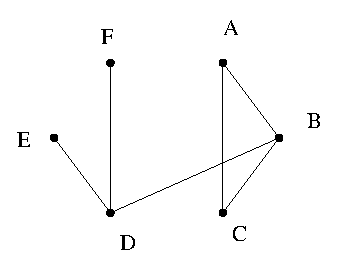
\includegraphics{figures/sample_graph.eps}%
\lthtmlpictureZ
\lthtmlcheckvsize\clearpage}

{\newpage\clearpage
\lthtmlfigureA{table1783}%
\begin{table}\begin{center}
\(\begin{array}{cccccc}
	  & B & C & D & E & F \\A & 1 & 1 & 0 & 0 & 0 \\B & & 1 & 1
	  & 0 & 0 \\C & & & 0 & 0 & 0 \\D & & & & 1 & 1 \\E & & & &
	  & 0
\end{array}\)

\end{center}
\end{table}%
\lthtmlfigureZ
\lthtmlcheckvsize\clearpage}

\stepcounter{section}
\stepcounter{subsection}
{\newpage\clearpage
\lthtmlinlinemathA{tex2html_wrap_indisplay4521}%
$\displaystyle \left(\vphantom{\sqrt{\frac {\left(\frac{V(V-1)}{2} -
(V-2)\right)\left(\frac{V(V-1)}{2} - (V-2)\right) }
{\left(\frac{V(V-1)}{2} - (V-2) - (V-2)\right)^{2}}}
}\right.$%
\lthtmlindisplaymathZ
\lthtmlcheckvsize\clearpage}

{\newpage\clearpage
\lthtmlinlinemathA{tex2html_wrap_indisplay4522}%
$\displaystyle \sqrt{{\frac {\left(\frac{V(V-1)}{2} -
(V-2)\right)\left(\frac{V(V-1)}{2} - (V-2)\right) }
{\left(\frac{V(V-1)}{2} - (V-2) - (V-2)\right)^{2}}}}$%
\lthtmlindisplaymathZ
\lthtmlcheckvsize\clearpage}

{\newpage\clearpage
\lthtmlinlinemathA{tex2html_wrap_indisplay4523}%
$\displaystyle \left.\vphantom{\sqrt{\frac {\left(\frac{V(V-1)}{2} -
(V-2)\right)\left(\frac{V(V-1)}{2} - (V-2)\right) }
{\left(\frac{V(V-1)}{2} - (V-2) - (V-2)\right)^{2}}}
}\right)$%
\lthtmlindisplaymathZ
\lthtmlcheckvsize\clearpage}

{\newpage\clearpage
\lthtmlfigureA{proof1812}%
\begin{proof}
There is a path from every vertex to vertex $V$, and there are $V-1$
edges, therefore the graph is a tree.  Trees are connected.
\end{proof}%
\lthtmlfigureZ
\lthtmlcheckvsize\clearpage}

{\newpage\clearpage
\lthtmlfigureA{proof1817}%
\begin{proof}
No graph with $V-2$\  edges is connected.
\end{proof}%
\lthtmlfigureZ
\lthtmlcheckvsize\clearpage}

{\newpage\clearpage
\lthtmlfigureA{proof1822}%
\begin{proof}
% latex2html id marker 1822

We apply Theorem \ref{th:amb}, we consider only simple undirected
graphs with $V \ge 3$. 
\par
Let $X$\  be the graphs whose adjacency matrix has exactly one 1 in each
row.  By Lemma \ref{lm:1erc} all such graphs are connected. Let $Y$\  be
the graphs in which there is exactly one 1 in each row of the
adjacency matrix, with the exception that one of the upper
$\left\lfloor(V-1)/2\right\rfloor$\  rows contains only 0's.  By Lemma
\ref{lm:1ernc} all such graphs are unconnected.
\par
For the relation $P$\  let $xPy$\  if and only if the graphs $x$\  and $y$
differ by one edge.  We immediately have $l = l' = 1$.  For each
element $x \in X$, if $y$\  is identical to $x$\  with the exception that
one of its first $\left\lfloor(V-1)/2\right\rfloor$\  rows contains all
$0$'s then $xPy$, so $m = \left\lfloor(V-1)/2\right\rfloor$.  A
similar argument leads to $m^{\prime} =
\left\lfloor(V-1)/2\right\rfloor + 1$\  if $V$\  is odd, and
$\left\lfloor(V-1)/2\right\rfloor + 2$\  if $V$\  is even.
\par
For simplicity take $m^{\prime} =
\left\lfloor(V-1)/2\right\rfloor$;  lowering
$m^{\prime}$\  can only worsen our result.  Theorem \ref{th:amb} now
implies a lower bound of
\begin{displaymath}\Omega\left(\sqrt{\frac{mm^{\prime}}{ll^{\prime}}}\right) = 
\Omega\left(\sqrt{\frac{\left\lfloor\frac{V-1}{2}\right\rfloor^{2}}{1}}\right) = 
\Omega\left(V\right) 
.\end{displaymath}
\end{proof}%
\lthtmlfigureZ
\lthtmlcheckvsize\clearpage}

{\newpage\clearpage
\lthtmlpictureA{tex2html_wrap4557}%
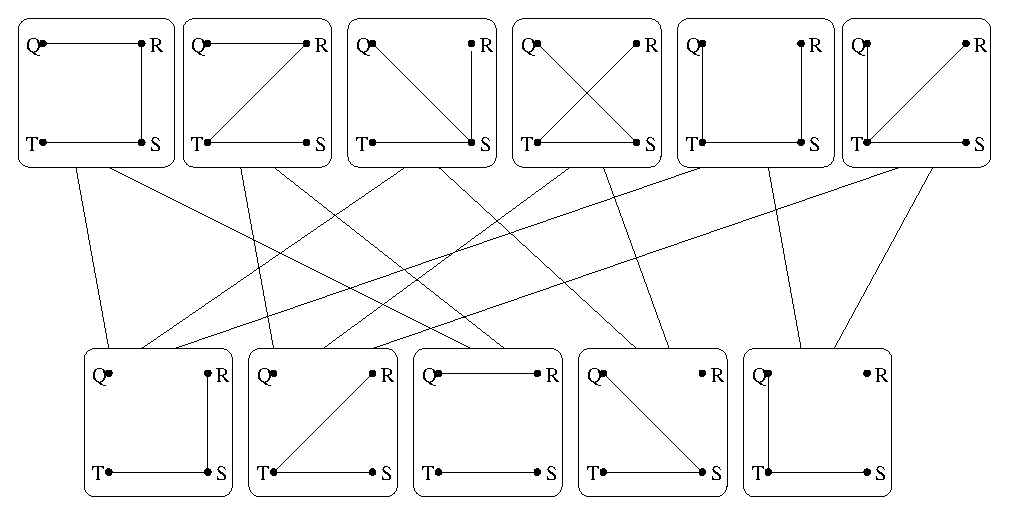
\includegraphics{figures/conn2.eps}%
\lthtmlpictureZ
\lthtmlcheckvsize\clearpage}

\stepcounter{subsection}
{\newpage\clearpage
\lthtmlfigureA{proof1852}%
\begin{proof}
% latex2html id marker 1852

We apply Lemma \ref{lm:1xky}, we will only consider simple undirected
graphs with $V \ge 3$.  
\par
Let $x$\  be the complete bipartite graph with the first $\left\lfloor
V/2 \right\rfloor$\  vertices and second $\left\lceil V/2 \right\rceil$
vertices forming the partitions.  Observe that adding any edge to $x$
results in a non-bipartite graph.  There are
\begin{displaymath}
\frac{V(V-1)}{2} - {\left\lfloor\frac{V}{2}\right\rfloor} {\left\lceil\frac{V}{2}\right\rceil} 
= \Theta(V^{2})
\end{displaymath}
such graphs, as there are $V(V-1)/2$\  possible edges, $\left\lfloor
V/2\right\rfloor \left\lceil V/2\right\rceil$\  of which are in $x$.
Lemma \ref{lm:1xky} implies the lower bound $\Omega(\sqrt{V^{2}}) =
\Omega(V)$.
\end{proof}%
\lthtmlfigureZ
\lthtmlcheckvsize\clearpage}

\stepcounter{section}
{\newpage\clearpage
\lthtmlinlinemathA{tex2html_wrap_inline4575}%
$ \Theta$%
\lthtmlinlinemathZ
\lthtmlcheckvsize\clearpage}



\newtheorem{cond}{Condition}[section]%



\newtheorem{algoi}{Algorithm}[section]%

\stepcounter{chapter}
\stepcounter{section}
{\newpage\clearpage
\lthtmlfigureA{proof2249}%
\begin{proof}
% latex2html id marker 2249

For any tree function $f$\  let $d$\  be the number of terms, and let
$c_{max}$\  be the maximum number of variables in any conjunction.
\par
The tree function $f$\  has a conjunctive term of size $c_{max}$.  Let
$x$\  be the input that gives every variable in that term the value 1,
and every other variable 0, so that $f(x) = 1$.  The inputs attained
by negating one of the $c_{max}$\  1's in $x$\  will yield $0$\  when
evaluated by $f$.  Lemma \ref{lm:1xky} implies that
$\Omega(\sqrt{c_{max}})$\  oracle queries are required to compute $f$.
\par
The tree function $f$\  also has $d$\  terms.  Let $x$\  be the input that
vices the first variable of every term the value 0 and every other
variable the value 1, so that $f(x) = 0$.  The inputs attained by
negating one of the $d$\  0's in $x$\  yield $1$\  when evaluated by $f$.
Lemma \ref{lm:1xky} now implies that $\Omega(\sqrt{d})$\  oracle queries
are required to compute $f$.
\par
Since $d \ge N/c_{max}$, either $c_{max} > \sqrt{N}$\  or $d \ge
\sqrt{N}$, and the theorem follows.
\end{proof}%
\lthtmlfigureZ
\lthtmlcheckvsize\clearpage}

\stepcounter{section}
{\newpage\clearpage
\lthtmlinlinemathA{tex2html_wrap_inline4653}%
$ \max_{{x}}^{}$%
\lthtmlinlinemathZ
\lthtmlcheckvsize\clearpage}

\stepcounter{section}
{\newpage\clearpage
\lthtmlfigureA{proof2300}%
\begin{proof}
% latex2html id marker 2300

We will prove that any nondeterministically evasive $N$-bit Boolean
function $f$\  has an input $x$\  such that for at least half of the
Hamming neighbors of $x$\  disagree with $x$\  when evaluated by $f$.
Once this is proved the theorem will follow from Lemma \ref{lm:1xky}.
\par
Assume to the contrary that for all inputs $x$\  more than half of $x$'s
Hamming neighbors agree with $x$.  Consider any deterministic decision
tree that computes $f$.  Since $D(f) \ge N(f) = N$, there is some path
$P$\  of length $N$\  in the tree.  Call the variables along this path $a,
b, \ldots , z$, where each label corresponds to a unique number
between 1 and N inclusive.  Let $x_{a}, x_{b}, \ldots , x_{z}$\  be the
values of the corresponding bits along the path.  Let us rearrange the
order of the input bits so that $a$\  is the first input bit, $b$\  is the
second input bit, and $z$\  is the $N$th input bit.  Then path $P$\  tells
us $f(x_{a}x_{b}\ldots x_{z})$\  is either $0$\  or $1$, and
$f(x_{a}x_{b}\ldots\overline{x_{z}})$\  is the other.  Without loss of
generality let $f(x_{a}x_{b}\ldots x_{z}) = 1$\  and
$f(x_{a}x_{b}\ldots\overline{x_{z}}) = 0$.
\par
By the pigeonhole principle, there is some bit $i < N-1$\  such that
\begin{displaymath}
\begin{array}{ll}
	f(x_{a}x_{b}\ldots x_{i}\ldots x_{z}) = 1 & 	f(x_{a}x_{b}\ldots x_{i} \ldots \overline{x_{z}}) = 0 \\
	f(x_{a}x_{b}\ldots\overline{x_{i}}\ldots x_{z}) = 1 & 	f(x_{a}x_{b}\ldots\overline{x_{i}}\ldots\overline{x_{z}}) = 0 .
\end{array}
\end{displaymath}
However, if this is the case then we do not need to ask about the
$i$th bit on path $P$.  This argument follows for any path of length
$N$\  in our deterministic decision tree.  In this case $D_{0}(f)$\  and
$D_{1}(f)$\  are at most $N-1$.  $N(f)$\  is then $N-1$, a contradiction
to the condition that $N(f) = N$.  Therefore our assumption was false,
and there is at least one input $x$\  such that at least half of $x$'s
Hamming neighbors yield a different value than $x$\  when evaluated by
$f$.  By Lemma \ref{lm:1xky} $\Omega(\sqrt{N})$\  oracle queries are
required to compute $f$\  in the bounded error setting.
\end{proof}%
\lthtmlfigureZ
\lthtmlcheckvsize\clearpage}

\stepcounter{section}
{\newpage\clearpage
\lthtmlfigureA{proof2350}%
\begin{proof}
% latex2html id marker 2350

By Lemma \ref{lm:1xky}, $\Omega(\sqrt{N(f)})$\  oracle queries are
required to compute any sensitive Boolean function. 
\par
Lov{\'{a}}sz and G{\'{a}}cs \cite{lovasz94complexity} proved that
$D(f) \le D_{0}(f) \cdot D_{1}(f)$, and by definition, $N(f) =
\max\{D_{0}(f),D_{1}(f)\}$.  Thus, $N(f) = \Omega(\sqrt{D(f)})$, 
and the theorem follows.
\end{proof}%
\lthtmlfigureZ
\lthtmlcheckvsize\clearpage}

{\newpage\clearpage
\lthtmlinlinemathA{tex2html_wrap_inline4692}%
$ \sqrt[6]{{D(f)}}$%
\lthtmlinlinemathZ
\lthtmlcheckvsize\clearpage}

\stepcounter{chapter}

\end{document}
